% Desenvolvido por Prof. Dr. David Buzatto
%
% Baseado na documentação do abntex2 e nos modelos em
% Microsoft Word propostos pela Profa. Dra. Rosana F. L. Rodrigues
% e pela bibliotecária M.Sc. Maria Carolina Gonçalves do campus
% São João da Boa Vista do IFSP.
%
% Versão 1.3
% Data: 09/08/2018

\documentclass[
	% -- opções da classe memoir --
	12pt,				% tamanho da fonte
	openright,			% capítulos começam em pág ímpar (insere página vazia caso preciso)
	twoside,			% para impressão em verso e anverso. Oposto a oneside
	a4paper,			% tamanho do papel. 
	%normalfigtabnum,
	%pnumromarab,
	% -- opções da classe abntex2 --
	chapter=TITLE,		% títulos de capítulos convertidos em letras maiúsculas
	section=TITLE,		% títulos de seções convertidos em letras maiúsculas
	%subsection=TITLE,	% títulos de subseções convertidos em letras maiúsculas
	%subsubsection=TITLE,% títulos de subsubseções convertidos em letras maiúsculas
	% -- opções do pacote babel --
	english,			% idioma adicional para hifenização
	french,				% idioma adicional para hifenização
	spanish,			% idioma adicional para hifenização
	brazil,				% o último idioma é o principal do documento
]{abntex2}






% ---------------------------------------------------------------------------------
%                                   PACOTES
% ---------------------------------------------------------------------------------

% ---
% Pacotes básicos 
% ---
\usepackage{lmodern}			% Usa a fonte Latin Modern			
\usepackage[T1]{fontenc}		% Selecao de codigos de fonte.
\usepackage[utf8]{inputenc}		% Codificacao do documento (conversão automática dos acentos)
\usepackage{lastpage}			% Usado pela Ficha catalográfica
\usepackage{indentfirst}		% Indenta o primeiro parágrafo de cada seção.
\usepackage{color}				% Controle das cores
\usepackage{graphicx}	% Inclusão de gráficos
\usepackage{microtype} 			% para melhorias de justificação
\usepackage{hyperref}
\usepackage{subfig}
\usepackage{epigraph}
\usepackage{url}
\usepackage{placeins}
\usepackage{multirow}
\usepackage[figuresright]{rotating}
\usepackage{chemfig}
\usepackage{amsmath}
\usepackage{amssymb}
\usepackage{enumitem}
\usepackage{bigints}
\usepackage{listings}
\usepackage{etoolbox}
\let\footruleskip\undefined
\usepackage[printwatermark]{xwatermark}
% ---

% ---
% Pacotes adicionais, usados apenas no âmbito do Modelo Canônico do abnteX2
% ---
\usepackage{lipsum}				% para geração de dummy text
% ---

% ---
% Pacotes de citações
% ---
\usepackage[brazilian,hyperpageref]{backref}	 % Paginas com as citações na bibl
\usepackage[alf,abnt-emphasize=bf]{abntex2cite}  % Citações padrão ABNT


% ---------------------------------------------------------------------------------
%                          CONFIGURAÇÕES DOS PACOTES
% ---------------------------------------------------------------------------------

% ---
% Configurações do pacote backref
%
% Para desativar, tire o comentário de \begin{comment} e \end{comment} 
% das próximas linhas e comente a linha \usepackage[brazilian,hyperpageref]{backref}
% acima.
% ---

%\begin{comment}
% ---
% Configurações do pacote backref
% Usado sem a opção hyperpageref de backref
\renewcommand{\backrefpagesname}{Citado na(s) página(s):~}
% Texto padrão antes do número das páginas
\renewcommand{\backref}{}
% Define os textos da citação
\renewcommand*{\backrefalt}[4]{
	\ifcase #1 %
	Nenhuma citação no texto.%
	\or
	Citado na página #2.%
	\else
	Citado #1 vezes nas páginas #2.%
	\fi}%
% ---
%\end{comment}


% listagens
\definecolor{corComentario}{RGB}{150,150,150}
\definecolor{corString}{RGB}{206,123,0}
\definecolor{corPalavraChave}{RGB}{0,0,230}

\lstset{
	numbers=left,
	stepnumber=1,
	firstnumber=1,
	numberstyle=\footnotesize,
	extendedchars=true,
	breaklines=true,
	lineskip=0pt,
	frame=tb,
	basicstyle=\ttfamily\footnotesize,
	showstringspaces=false,
	stringstyle=\color{corString},
	commentstyle=\color{corComentario},
	keywordstyle=\color{corPalavraChave}
}

\newcolumntype{Y}{>{\centering\arraybackslash}X}

\newcommand{\ano}[1]{\def \oano {#1}}
\newcommand{\imprimirano}{\oano}

\newcommand{\mes}[1]{\def \omes {#1}}
\newcommand{\imprimirmes}{\omes}

\newcommand{\subtitulo}[1]{\def \osubtitulo {#1}}
\newcommand{\imprimirsubtitulo}{\osubtitulo}

\newcommand{\area}[1]{\def \aarea {#1}}
\newcommand{\imprimirarea}{\aarea}

\renewcommand{\coorientador}[1]{\def \ocoorientador {#1}}
\renewcommand{\imprimircoorientador}{\ocoorientador}

\newcommand{\grau}[1]{\def \ograu {#1}}
\newcommand{\imprimirgrau}{\ograu}

\newcommand{\curso}[1]{\def \ocurso {#1}}
\newcommand{\imprimircurso}{\ocurso}

\newwatermark*[page=4,color=red!50,angle=60,scale=2,xpos=-20,ypos=20]{ALUNO:\\SUBSTITUIR PELA\\FICHA DA\\BIBLIOTECA}
\newwatermark*[page=5,color=blue!50,angle=60,scale=2,xpos=0,ypos=0]{COORDENADOR:\\SUBSTITUIR PELA\\FOLHA DE\\APROVAÇÃO}

% ---
% Informações de dados para CAPA e FOLHA DE ROSTO
% ---

\curso{Tecnologia em Automação Industrial}
\grau{}

%exemplos
%\curso{Tecnologia em Sistemas para Internet}
%\grau{Tecnólogo em Sistemas para Internet}
%\curso{Especialização em Desenvolvimento de Aplicações para Dispositivos Móveis}
%\grau{Especialista em Desenvolvimento de Aplicações para Dispositivos Móveis}

\titulo{Analise de arranjos fotovoltaicos através do uso de MPPT}

% caso não haja subtítulo, comente a linha abaixo
%\subtitulo{subtítulo}

\tipotrabalho{Trabalho de Conclusão de Curso}
\area{Área de Concentração do Trabalho}

\autor{Murilo Fabricio Silva\and Victor Hugo Dias Lopes}
\orientador{Prof.Dr. Marcelo Kenji Shibuya}

% caso não haja coorientador, comente a linha abaixo
%\coorientador{Prof./Profa. Me./Dr./Dra. Nome Completo}

\local{Guarulhos}
\mes{MÊS}
\ano{2019}

\instituicao{%
	Instituto Federal de Educação, Ciência e Tecnologia de São Paulo
	\par
	Câmpus Guarulhos
}

\preambulo{\imprimirtipotrabalho\ apresentado ao Instituto Federal de Educação, Ciência e Tecnologia de São Paulo, como parte dos requisitos para a obtenção do grau de tecnologo em automação industrial \imprimirgrau.
\\
\\
\\
\\
}
%Área de Concentração: \imprimirarea}
% ---


% ---
% Configurações de aparência do PDF final
% ---

% alterando o aspecto da cor azul
\definecolor{blue}{RGB}{41,5,195}

% informações do PDF
\makeatletter
\hypersetup{
	%pagebackref=true,
	pdftitle={\@title}, 
	pdfauthor={\@author},
	pdfsubject={\imprimirpreambulo},
	pdfcreator={Murilo Fabricio Silva},
	pdfkeywords={Palavra chave 1}{Palavra chave 2}{Palavra chave 3}{Palavra chave n}, 
	colorlinks=true,       		% false: boxed links; true: colored links
	linkcolor=black,          	% color of internal links
	citecolor=black,       		% color of links to bibliography
	filecolor=black,      		% color of file links
	urlcolor=black,
	bookmarksdepth=4
}
\makeatother
% --- 


% ---
% Comandos do autor
% ---

% comando para inserir autor e ano
\newcommand{\citeauthorandyear}[1]{\citeauthoronline{#1} (\citeyear{#1})}


% ---
% Novo list of (listings) para Quadros
% ---

\newcommand{\quadroname}{Quadro}
\newcommand{\listofquadrosname}{Lista de Quadros}

\newfloat[chapter]{quadro}{loq}{\quadroname}
\newlistof{listofquadros}{loq}{\listofquadrosname}
\newlistentry{quadro}{loq}{0}

% configurações para atender às regras da ABNT
\setfloatadjustment{quadro}{\centering}
\counterwithout{quadro}{chapter}
\renewcommand{\cftquadroname}{\quadroname\space} 
\renewcommand*{\cftquadroaftersnum}{\hfill--\hfill}

% Configuração de posicionamento padrão:
\setfloatlocations{quadro}{hbtp}



% --- 
% Espaçamentos entre linhas e parágrafos 
% --- 

% O tamanho do parágrafo é dado por:
\setlength{\parindent}{1.3cm}

% Controle do espaçamento entre um parágrafo e outro:
\setlength{\parskip}{0.2cm}  % tente também \onelineskip

% ---
% compila o indice
% ---
\makeindex
% ---







% ---------------------------------------------------------------------------------
%                                   INÍCIO DO DOCUMENTO
% ---------------------------------------------------------------------------------
\begin{document}
	
% Seleciona o idioma do documento (conforme pacotes do babel)
%\selectlanguage{english}
\selectlanguage{brazil}

% Retira espaço extra obsoleto entre as frases.
\frenchspacing 


% ---------------------------------------------------------------------------------
%                                   ELEMENTOS PRÉ-TEXTUAIS
% ---------------------------------------------------------------------------------
% \pretextual

% ---
% Capa
% ---
%\imprimircapa
% capa personalizada

\begin{center}
	
	%\center
	\ABNTEXchapterfont\Large\textsc{\imprimirinstituicao}
	\vspace{3.5cm}
	
    \ABNTEXchapterfont\Large\textsc{\imprimirautor}
	\vspace{3.5cm}
	
    \ABNTEXchapterfont\LARGE\textsc{\imprimirtitulo\ifdef{\osubtitulo}{:}{}}
    
    \ifdef{\osubtitulo}{\ABNTEXchapterfont\Large\imprimirsubtitulo}{}
	\vfill
	
	\Large\textsc{\imprimirlocal}
	
	\Large\textsc{\imprimirano}
	
	\vspace*{2cm}
	
\end{center}

\cleardoublepage


% ---

% ---
% Folha de rosto
% (o * indica que haverá a ficha bibliográfica)
% ---
%\imprimirfolhaderosto*
\begin{center}
   	
   	\ABNTEXchapterfont\Large\textsc{\imprimirautor}
   	\vspace{2.5cm}
   	
    \ABNTEXchapterfont\LARGE\imprimirtitulo\ifdef{\osubtitulo}{:}{}
                           
    \ifdef{\osubtitulo}{\ABNTEXchapterfont\Large\imprimirsubtitulo}{}
   	\vspace{2.5cm}
   	   	
   	\hspace{.4\textwidth}
   	\begin{minipage}{.5\textwidth}
   		\SingleSpacing
   		\large\imprimirpreambulo
   		
   		\vspace{\onelineskip}
   		
   		Orientador: \imprimirorientador
   		
        \ifdef{\ocoorientador}{
     		\vspace{\onelineskip}
   		
    		Coorientador: \imprimircoorientador
        }{}
   		
   	\end{minipage}%
    \vfill
   	
   	\Large\textsc{\imprimirlocal}
   	
   	\Large\textsc{\imprimirano}
   	
   	\vspace*{2cm}
   	
\end{center}
% ---

% ---
% Inserir a ficha catalográfica
% ---
% Isto é um exemplo de Ficha Catalográfica, ou ``Dados internacionais de
% catalogação-na-publicação''. Você pode utilizar este modelo como referência. 
% Porém, provavelmente a biblioteca da sua universidade lhe fornecerá um PDF
% com a ficha catalográfica definitiva após a defesa do trabalho. Quando estiver
% com o documento, salve-o como PDF no diretório do seu projeto e substitua todo
% o conteúdo de implementação deste arquivo pelo comando abaixo:
%
% \begin{fichacatalografica}
%     \includepdf{fig_ficha_catalografica.pdf}
% \end{fichacatalografica}

\begin{fichacatalografica}
	
	Folha destinada à inclusão da Catalogação na Fonte - Ficha Catalográfica (a ser solicitada à Biblioteca IFSP – Câmpus São João da Boa Vista e posteriormente impressa no verso da Folha de Rosto (folha anterior).
	
	\vspace{3cm}
	
	\begin{center}
		Catalogação na Fonte preparada pela Biblioteca Comunitária “Wolgran Junqueira Ferreira” do IFSP – Câmpus São João da Boa Vista
	\end{center}
	
	
	\sffamily
	\vspace*{\fill}					% Posição vertical
	\begin{center}					% Minipage Centralizado
		\fbox{\begin{minipage}[c][8cm]{13.5cm}		% Largura
			\small
			\imprimirautor
			%Sobrenome, Nome do autor
			
			\hspace{0.5cm} \imprimirtitulo  / \imprimirautor. --
			\imprimirlocal, \imprimirano-
			
			\hspace{0.5cm} \pageref{LastPage} p. : il. (algumas color.) ; 30 cm.\\
			
			\hspace{0.5cm} Orientador ~Prof. Dr. \imprimirorientador\\
			
			\hspace{0.5cm}
			\parbox[t]{\textwidth}{\imprimirtipotrabalho~--~\imprimirinstituicao,
				\imprimirano.}\\
			
			\hspace{0.5cm}
			1. Palavra-chave 1.
			2. Palavra-chave 2.
			3. Palavra-chave 3.
			I. Orientador.
			II. Instituto Federal de Educação, Ciência e Tecnologia de São Paulo.
			III. Título 			
		\end{minipage}}
	\end{center}
\end{fichacatalografica}

% ---
% Inserir folha de aprovação
% ---
% Isto é um exemplo de Folha de aprovação, elemento obrigatório da NBR
% 14724/2011 (seção 4.2.1.3). Você pode utilizar este modelo até a aprovação
% do trabalho. Após isso, substitua todo o conteúdo deste arquivo por uma
% imagem da página assinada pela banca com o comando abaixo:
%
% \includepdf{folhadeaprovacao_final.pdf}
%
\begin{folhadeaprovacao}
	
	\begin{center}
		
		{\ABNTEXchapterfont\large\textsc{\imprimirautor}}
		
		\vspace*{\fill}\vspace*{\fill}
		\begin{center}
            \ABNTEXchapterfont\Large\textsc{\imprimirtitulo\ifdef{\osubtitulo}{:}{}}
            
            \ifdef{\osubtitulo}{\ABNTEXchapterfont\Large\imprimirsubtitulo}{}
		\end{center}
		\vspace*{\fill}
		
		\hspace{.45\textwidth}
		\begin{minipage}{.5\textwidth}
			\imprimirpreambulo
		\end{minipage}%
		\vspace*{\fill}
	\end{center}
	
	Aprovado em DIA(número) de MÊS(por extenso) de ANO(Número).
	
	\assinatura{\textbf{\imprimirorientador} \\ Orientador \\ Titulação \\ Instituição} 
	\assinatura{\textbf{Professor Convidado 1} \\ Titulação \\ Instituição}
	\assinatura{\textbf{Professor Convidado 2} \\ Titulação \\ Instituição}
	
	\begin{center}
		\vspace*{0.5cm}
		{\large\imprimirlocal}
		\par
		{\large\imprimirano}
		\vspace*{1cm}
	\end{center}
	
\end{folhadeaprovacao}

% ---
% Dedicatória
% ---
\begin{dedicatoria}
	\vspace*{\fill}
	\centering
	\noindent
	\textit{Dedicatória (Opcional). Não digite a palavra Dedicatória. Texto no qual o autor do trabalho oferece homenagem ou dedica o seu trabalho a alguém (não usar ponto final)}
    \vspace*{\fill}
\end{dedicatoria}

% ---
% Agradecimentos
% ---
\begin{agradecimentos}
	Agradecimento (opcional). Folha que contém manifestação de reconhecimento a pessoas e/ou instituições que realmente contribuíram com o autor, devendo ser expressos de maneira simples.	
\end{agradecimentos}

% ---
% Epígrafe
% ---
\begin{epigrafe}
	
	\vspace*{\fill}
	Epígrafe (Opcional) 
    Pensamentos retirados de um livro, uma música, um poema, normalmente relacionado ao tema do trabalho, seguida de indicação de autoria. As epígrafes podem ser colocadas também nas folhas de abertura de cada capítulo.  
    
	\epigraph{``\emph{Any fool can write code that a computer can understand. Good programmers write code that humans can understand}''.}{Martin Fowler}
	
\end{epigrafe}

% ---
% Resumos
% ---
\noindent{SOBRENOME, Prenome. \textbf{Título do trabalho de TCC colocado em negrito:} subtítulo (se houver). Ano da defesa. Tipo de documento (Grau e vinculação acadêmica) – Instituição, Local. Ano da entrega.}

\noindent{Exemplo: RODRIGUES, Rosana Ferrareto Lourenço. \textbf{Verbos de movimento em inglês:} uma proposta de descrição e ensino por meio do modelo de integração conceptual. 2012. Tese (Doutorado em Linguística e Língua Portuguesa) – Faculdade de Ciências e Letras, Câmpus Araraquara, Universidade Estadual Paulista, Arararaqua. 2012.}


\setlength{\absparsep}{18pt} % ajusta o espaçamento dos parágrafos do resumo
\begin{resumo}
	
	Elemento obrigatório, constituído de uma sequência de frases concisas e objetivas, fornecendo uma visão rápida e clara do conteúdo do estudo. O texto deverá conter entre 150 a 250 palavras e ser antecedido pela referência do estudo. Também, não deve conter citações e deverá ressaltar o objetivo, o método, os resultados e as conclusões. O resumo deve ser redigido em parágrafo único, seguido das palavras representativas do conteúdo do estudo, isto é, palavras-chave, em número de três a cinco, separadas entre si por ponto e finalizadas também por ponto. Usar o verbo na terceira pessoa do singular, com linguagem impessoal (pronome SE), bem como fazer uso, preferencialmente, da voz ativa.
	
	\vspace{\onelineskip}
	
	\textbf{Palavras-chave}: Palavra-chave 1. Palavra-chave 2. Palavra-chave 3. Palavra-chave n.
\end{resumo}
\noindent{SOBRENOME, Prenome. \textbf{Título do trabalho de TCC colocado em negrito:} subtítulo (se houver). Ano da defesa. Tipo de documento (Grau e vinculação acadêmica) – Instituição, Local. Ano da entrega.}

% resumo em inglês
\begin{resumo}[Abstract]
	\begin{otherlanguage*}{english}
		
		Elemento obrigatório. É a versão do resumo em português para o idioma de divulgação internacional. Deve ser antecedido pela referência do estudo.
		
		\vspace{\onelineskip}
		 
		\textbf{Keywords}: Keyword 1. Keyword 2. Keyword 3. Keyword n.
	\end{otherlanguage*}
\end{resumo} 

% ---
% inserir lista de ilustrações
% ---
\pdfbookmark[0]{\listfigurename}{lof}
\listoffigures*
\cleardoublepage
% ---

% ---
% inserir lista de tabelas
% ---
\pdfbookmark[0]{\listtablename}{lot}
\listoftables*
\cleardoublepage
% ---

% ---
% inserir lista de quadros
% ---
\pdfbookmark[0]{\listofquadrosname}{loq}
\listofquadros*
\cleardoublepage
% ---

% ---
% inserir lista de abreviaturas e siglas
% ---
\begin{siglas}
	\item[1D] Uma dimensão
	\item[2D] Duas dimensões
	\item[3D] Três dimensões
\end{siglas}
% ---

% ---
% inserir lista de símbolos
% ---
\begin{simbolos}
	\item[$\alpha$] Letra grega minúscula Alfa
	\item[$\beta$] Letra grega minúscula Beta
\end{simbolos}
% ---

% ---
% inserir o sumário
% ---
\pdfbookmark[0]{\contentsname}{toc}
\tableofcontents*
\cleardoublepage
% ---






% ---------------------------------------------------------------------------------
%                                  ELEMENTOS TEXTUAIS
% ---------------------------------------------------------------------------------
\textual

\chapter{Introdução}
\label{cap:01}
A energia tem se tornado cada vez mais importante no mundo atual, assim como a busca de meios de energias renováveis e sustentáveis. Entre as principais formas de geração de energia no Brasil são citáveis as energias eólica e solar, que com o avanço da tecnologia têm se tornado cada vez mais acessível. No Brasil, há grande potencial de geração de energia solar, devido a sua posição geográfica, próximo a linha do Equador. Entre as formas de energia solar, o uso da energia fotovoltaica têm se tornado mais popular. Entretanto, para garantir que um sistema que utilize energia fotovoltaica seja viável é necessário o uso de alguns processos que permitam uma geração eficiente, como o uso MPPT, \textit{Maximum Power Point Tracker}, ou Rastreador de Máxima Potência, de forma a garantir que o sistema dê a maior potência possível em um determinado período.

\indent		Tendo este aspecto em mente, este trabalho terá como premissa o desenvolvimento de uma metodologia de análise de sistemas fotovoltaicos a partir do uso do MPPT, de maneira a garantir e viabilizar o uso de sistemas fotovoltaicos que sejam compactos, eficazes e baratos.
Logo, através de um sistema que gera dados que disponibilizem o modo de atuação de um sistema fotovoltaico, é possível encontrar o ponto de máxima potência e gerar diversos gráficos a respeito do mesmo, assim permitindo uma análise completa e a comparação com diversos sistemas.


\section{Justificativa}

No Brasil, cerca de 81,9\% da capacidade de geração de energia e 87,8\% da produção total foram por meio de energias renováveis, sendo a matriz hidráulica ainda dominante com 63,7\%, e tendo 8,1\% as usinas eólicas e 1\% as solares, em junho de 2018 de acordo com o Boletim de Monitoramento do Sistema Elétrico, divulgado pelo Ministério de Minas e energias.%ADICIONAR REFERÊNCIA

\indent	Nota-se que a energia solar ainda está se popularizando no Brasil, entretanto segundo a Organização das Nações Unidas(ONU), os investimentos focados em energia solar já ultrapassam a casa dos US\$ 160 bilhões, se tornando cada vez mais importantes em um contexto de geração de energia sustentável. Dito isso, há a necessidade de engajar o uso e conhecimento deste meio de geração de energia, desta maneira, permitindo ao país a diversificação de suas fontes de geração elétrica, de maneira a permitir maior flexibilidade e uma menor dependência a apenas um meio.
Realidade a qual pode gerar diversas consequências em caso de problemas ou falta na geração a partir desse meio, como aumento das taxas pagas sobre o consumo de energia, desencadeando diversos problemas econômicos, sociais, e estruturais sobre um país. Entretanto, ao estimular o uso da energia solar é possível descentralizar as fontes de geração de energia por meio de um meio de geração limpo, sustentável, e viável, gerando diversas oportunidades de geração de trabalho e estudo.%ADICIONAR REFERÊNCIA


\section{Objetivos}

\subsection{Objetivo Geral}

Analisar o comportamento de painéis fotovoltaicos por meio do uso de sua curva I-V.

\subsection{Objetivos Específicos}
\begin{itemize}
	\item Desenvolver um sistema traçador de curva I-V de baixo custo;
	\item Comparar curvas I-V durante diferentes níveis de irradiação solar em diferentes painéis fotovoltaicos;
	\item Valorizar o uso de sistemas fotovoltaicos para estudo e uso em faculdades e empresas ao redor do Brasil;
	\item Categorizar usos diversos de sistemas traçadores de curva I-V para diferentes aplicações para estudo ou comercialmente.

\end{itemize}

\section{Metodologia}

A metodologia utilizada durante a realização do trabalho tem como base o tipo de pesquisa tecnológica exploratória, de maneira a descrever e desenvolver a curva I-V de um painel fotovoltaico e seu uso em estudos ou uso comercial. Deste modo foram realizados os seguintes passos:1.Análise bibliográfica; 2.Desenvolvimento de um sistema protótipo; 3.Teste do circuito; 4.Análise dos dados coletados; 5.Teste para diferentes quantidades de conjuntos de valores. 6.Comparação e análise dos dados coletados, gráficos gerados e curva teórica.

\chapter{Revisão da Literatura}
\label{cap:02}

Texto da revisão da literatura, dividido em seções e subseções.


Este é um exemplo de como usar figuras. Referência cruzada: Figura~\ref{fig:exemplo}

\FloatBarrier
\begin{figure}[!htbp]
	\centering
	\caption{Exemplo de figura}
	%scale redimensiona a figura.
	%1.5 = 150% do tamanho original
	%1 = 100% do tamanho original
	%0.20 = 20% do tamanho original
	
\includegraphics[scale=1.5]{imagens/exemploFigura}
	\\\textbf{Fonte:} Elaborada pelo autor
	\label{fig:exemplo}
\end{figure}
\FloatBarrier


Este é um exemplo de como usar tabelas. Referência cruzada: Tabela~\ref{tab:exemplo}

\FloatBarrier
\begin{table}[!htbp]
\centering
\caption{Exemplo de tabela de 2 colunas}
	\begin{tabular}{ c | c }
		\hline
		\textbf{Coluna 1} & \textbf{Coluna 2} \\ \hline
		Dado 1a           & Dado 1b           \\ \hline
		Dado 2a           & Dado 2b           \\ \hline
		Dado 3a           & Dado 3b           \\ \hline
		Dado 4a           & Dado 4b           \\ \hline
	\end{tabular}
	\\ \vspace{0.2cm}
	\textbf{Fonte:} Elaborada pelo autor
	\label{tab:exemplo}
\end{table}
\FloatBarrier


Este é um exemplo de como usar quadros. Referência cruzada: Quadro~\ref{qua:exemplo}

\FloatBarrier
\begin{quadro}[!htbp]
	\centering
	\caption{Exemplo de quadro}
	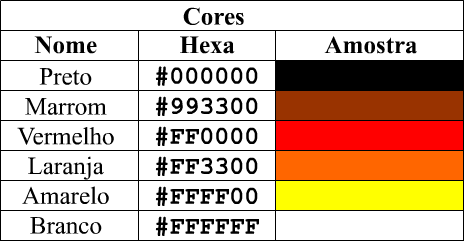
\includegraphics[scale=.7]{imagens/exemploQuadro}
	\\\textbf{Fonte:} Elaborada pelo autor
	\label{qua:exemplo}
\end{quadro}
\FloatBarrier


Este é um exemplo de como usar equações. Referência cruzada: Equação~\ref{eq:exemplo}

\begin{equation}
\sum_{i=1}^{n} = \frac{n(n+1)}{2}
\label{eq:exemplo}
\end{equation}


Exemplo de inserção de lista de código fonte (\textbf{\textcolor{red}{não use acentos no código!}}):

\lstinputlisting[language=Java]{fontes/ClasseExemplo.java} 



Este é um exemplo de como inserir texto sem formatação (ambiente verbatim):

\begin{verbatim}
	Texto sem formatação, como espaçamento igual.
\end{verbatim}


Exemplo de lista de itens:

\begin{itemize}
	\item \textbf{Item 1:} texto...;
	\item \textbf{Item 2:} texto...;
    \begin{itemize}
            \item \textbf{Subitem:} texto...;
            \item \textbf{Subitem:} texto...;
            \item \textbf{Subitem:} texto...;
        \end{itemize}
	\item \textbf{Item 3:} texto...;
	\item \textbf{Item n:} texto....
\end{itemize}


Exemplo de lista numerada:

\begin{enumerate}
	\item \textbf{Item:} texto...;
	\item \textbf{Item:} texto...;
    \begin{enumerate}
        \item \textbf{Subitem:} texto...;
        \item \textbf{Subitem:} texto...;
        \item \textbf{Subitem:} texto...;
    \end{enumerate}
	\item \textbf{Item:} texto...;
	\item \textbf{Item:} texto....
\end{enumerate}


Exemplos de comandos para texto e referências:

\begin{itemize}
	\item Para iniciar um novo parágrafo, basta deixar uma linha em branco no código fonte;
	\item Não force o compilador a pular mais de uma linha, pois terá influência negativa na composição do documento;
	\item Sempre deixe o \LaTeX\ realizar a formatação de parágrafos e posicionamento de elementos;
	\item Utilização de aspas simples (abertura \verb|`|, fechamento \verb|'|): `Texto entre aspas simples';
	\item Utilização de aspas duplas (abertura \verb|``|, fechamento \verb|''|): ``Texto entre aspas duplas'';
	\item Negrito (comando \verb|\textbf|): \textbf{texto em negrito};
	\item Itálico (comando \verb|\textit|): \textit{texto em itálico};
	\item Sublinhado (comando \verb|\underline|): \underline{texto sublinhado};
	\item Negrito e itálico (usar comandos juntos): \textbf{\textit{texto em negrito e itálico}};
	\item Alterar cor do texto (comando \verb|\textcolor{cor}{texto}|):
	\begin{itemize}
		\item Exemplo \verb|\textcolor{red}{texto}|: \textcolor{red}{texto vermelho};
		\item Exemplo \verb|\textcolor[RGB]{255, 102, 0}|: \textcolor[RGB]{255, 102, 0}{texto laranja};
		\item Exemplo \verb|\textcolor[HTML]{006AD7}|: \textcolor[HTML]{006AD7}{texto azul};
	\end{itemize}
	\item Ambiente matemático inline (comando \verb|$ expressão $|): $s = x^2-2x +1$;
	\item Referência normal (comando \verb|\cite|):
	\begin{itemize}
		\item \cite{Agaisse1995};
		\item \cite{Abedi2014};
		\item \cite{BtNomenclature2016};
	\end{itemize}
	\item Referência normal com mais de uma obra (comando \verb|\cite|):
	\begin{itemize}
		\item \cite{Agaisse1995, Abedi2014};
		\item \cite{Nelson2014, BtNomenclature2016, AgapitoTenfen2014};
	\end{itemize}
	\item Referência nome e ano (comando \verb|\citeauthorandyear|):
	\begin{itemize}
		\item \citeauthorandyear{Agaisse1995};
		\item \citeauthorandyear{Abedi2014};
		\item \citeauthorandyear{BtNomenclature2016};
	\end{itemize}
\end{itemize}


Exemplo 1 de referência direta:

\begin{citacao}
	Os 20 aminoácidos usualmente encontrados como resíduos em proteínas contém um grupo $\alpha$-carboxil, um grupo $\alpha$-amino e um grupo R distinto substituído no átomo de carbono $\alpha$. O átomo de carbono $\alpha$ de todos os aminoácidos, com exceção da glicina, é assimétrico e, portanto, os aminoácidos podem existir em pelo menos duas formas estereoisoméricas. Somente os estereoisômeros L, com uma configuração relacionada à configuração absoluta da molécula de referência L-gliceraldeído, são encontrados em proteínas \cite[p. 81]{Nelson2014}
\end{citacao}

Exemplo 2 de referência direta:

\begin{citacao}
	\textit{These various insecticidal proteins are synthesized during the stationary phase and accumulate in the mother cell as a crystal inclusion which can account for up to 25\% of the dry weight of the sporulated cells. The amount of crystal protein produced by a B. thuringiensis culture in laboratory conditions (about 0.5 mg of protein per ml) and the size of the crystals (24) indicate that each cell has to synthesize $10^6$ to $2 \times 10^6$ $\delta$-endotoxin molecules during the stationary phase to form a crystal} \cite[p. 1]{Agaisse1995}
\end{citacao}

Exemplo de nota de rodapé\footnote{Essa é uma nota de rodapé!}.

\chapter{Materiais e Métodos}
\label{cap:03}
Para a aquisição de dados foram utilizados diversos conceitos e ferramentas eletrônicas de diversas esferas específicas, garantindo uma melhor adaptação para o objetivo específico de traçador IxV.%ADICIONAR REFERÊNCIAS SOBRE O PROTÓTIPO

\section{Arduino}
Arduino, plataforma \textit{open-source}, baseada em fácil prototipagem eletrônica e de programação, permite o fácil e rápido desenvolvimento de protótipos. Devido a fácil disponibilidade no mercado e alto custo x benefício, fez-se o uso do Arduino Uno como componente principal para o controle e aquisição de dados para a curva IxV.

\FloatBarrier
\begin{figure}[!htbp]
	\centering
	%scale redimensiona a figura.
	%1.5 = 150% do tamanho original
	%1 = 100% do tamanho original
	%0.20 = 20% do tamanho original
	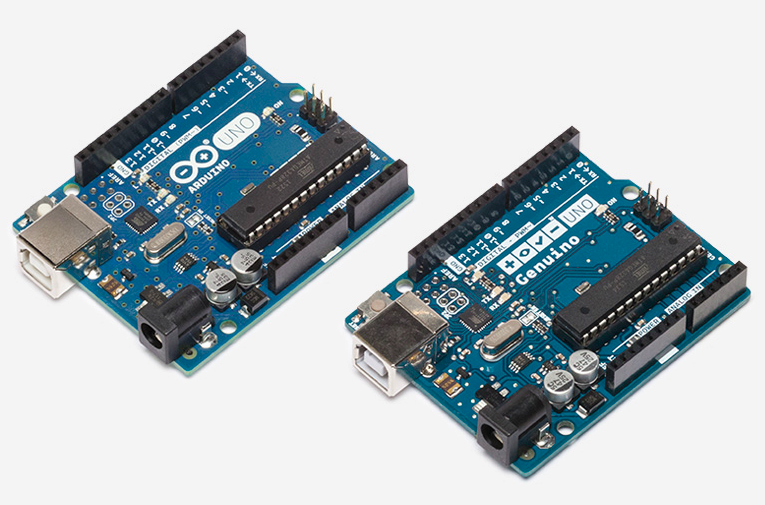
\includegraphics[scale=0.7]{imagens/Uno}
	\caption{Exemplos de Arduinos Uno. Fonte:  \url{https://www.arduino.cc/en/Guide/ArduinoUno}. }
	
	\label{fig:ArduinoUno}
\end{figure}
\FloatBarrier

Na Tabela 2 São Listadas as principais características encontradas no hardware do Arduino Uno.

\FloatBarrier
\begin{table}[!htbp]
	\centering
	\caption{Tabela do hardware do Arduino Uno}
	\begin{tabular}{ c | c }
		\hline
		Microcontrolador                & ATmega328P                                            \\ \hline
		Tensão operacional              & 5V                                                    \\ \hline
		Tensão de entrada (recomendado) & 7-12V                                                 \\ \hline
		Pinos Digital I / O             & 6-20V                                                 \\ \hline
		PWM Digital I / O Pins          & 6                                                     \\ \hline
		Pinos de entrada analógica      & 6                                                     \\ \hline
		Corrente DC por pino de E / S   & 20 mA                                                 \\ \hline
		Corrente DC para Pin 3.3V       & 50 mA                                                 \\ \hline
		Memória flash                   & 32 KB (ATmega328P) \\ \hline
		SRAM                            & 2 KB (ATmega328P)                                     \\ \hline
		EEPROM                          & 1 KB (ATmega328P)                                     \\ \hline
		Velocidade do relógio           & 16 MHz                                                \\ \hline
		LED BUILTIN                     & 13                                                    \\ \hline
		comprimento                     & 68.6 mm                                               \\ \hline
		Largura                         & 53.4 mm                                               \\ \hline
		Peso                            & 25 g                                                  \\ \hline
	\end{tabular}
	\\ \vspace{0.2cm}
	\textbf{Fonte:} Adaptado de \url{https://store.arduino.cc/usa/arduino-uno-rev3} .
	\label{tab:ArduinoUno}
\end{table}
\FloatBarrier

Conforma mostrado na tabela~\ref{tab:ArduinoUno}, o Arduino Uno possui 6 entradas analógicas, entretanto há grande imprecisão nestas entradas. De forma a garantir maior precisão nas coletas de dados, foi utilizado um modulo conversor analógico.

\section{ADS1115}
O módulo ADS1115 da Adafruit é um módulo ADC com resolução de 16-Bits e utiliza a comunicação I2C, o uso deste módulo foi vital para a aquisição de dados.

Diferentemente dos conversores Analógico Digital integrados na placa Arduino, o módulo ADS1115 possui ótima repetibilidade e grande precisão durante a a aquisição dos valores.

Há ainda a possibilidade do uso de amplificadores internos através de FPGA de forma a aumentar ainda mais a precisão das medidas.

Ao se utilizar sua resolução de 16-Bits, e ganho unitário é possível obter-se uma precisão de 0,125 $mV$, o qual ultrapassa grandemente o fundo de escala de 4,9 $mV$ do ADC proveniente do Arduino.%ADICIONAR REFERÊNCIA DE ONDE TIROU OS DADOS
\FloatBarrier
\begin{figure}[!htbp]
	\centering
	%scale redimensiona a figura.
	%1.5 = 150% do tamanho original
	%1 = 100% do tamanho original
	%0.20 = 20% do tamanho original
	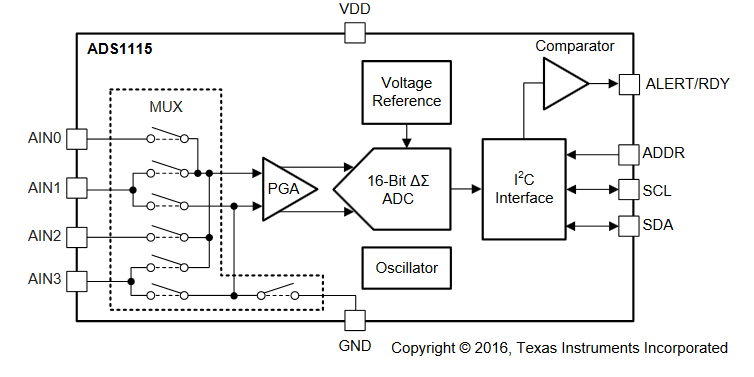
\includegraphics[scale=0.7]{imagens/ADS}
	\caption{Diagrama de blocos. Fonte: Datasheet do fabricante. }%ADICIONAR DATASHEET COM OS DADOS DO ARDUINO.
	
	\label{fig:Ads}
\end{figure}
\FloatBarrier

\chapter{Resultados e Discussão}
\label{cap:04}

Texto dos resultados.
\chapter{Conclusões/Conclusões Parciais}
\label{cap:05}

Texto das conclusões (as conclusões parciais são para a graduação na qualificação).

\chapter{Cronograma}
\label{cap:06}

Cronograma (para a graduação na qualificação)






% ---------------------------------------------------------------------------------
%                                 ELEMENTOS PÓS-TEXTUAIS
% ---------------------------------------------------------------------------------
\postextual


% ----------------------------------------------------------
% Referências bibliográficas
% ----------------------------------------------------------
\bibliography{referencias}


% ----------------------------------------------------------
% Glossário
% ----------------------------------------------------------
%
% Consulte o manual da classe abntex2 para orientações sobre o glossário.
%
%\glossary


% ----------------------------------------------------------
% Apêndices
% ----------------------------------------------------------
% texto ou documento elaborado pelo autor, a fim de complementar sua argumentação, sem prejuízo da unidade nuclear do trabalho,

% ---
% Inicia os apêndices
% ---
\begin{apendicesenv}
	
	% Imprime uma página indicando o início dos apêndices
	\partapendices
	
	% ----------------------------------------------------------
	\chapter{Título do Apêndice A}
	% ----------------------------------------------------------
	
	Texto do apêndice A.
	
	% ----------------------------------------------------------
	\chapter{Título do Apêndice B}
	% ----------------------------------------------------------
	
	Texto do apêndice B.
	
\end{apendicesenv}
% ---


% ----------------------------------------------------------
% Anexos
% ----------------------------------------------------------
% texto ou documento não elaborado pelo autor, que serve de fundamentação, comprovação e ilustração.

% ---
% Inicia os anexos
% ---
\begin{anexosenv}
	
	% Imprime uma página indicando o início dos anexos
	\partanexos
	
	% ----------------------------------------------------------
	\chapter{Título do Anexo A}
	% ----------------------------------------------------------
	
	Texto do anexo A.
	
	% ----------------------------------------------------------
	\chapter{Título do Anexo B}
	% ----------------------------------------------------------
	
	Texto do anexo B.
	
\end{anexosenv}


%---------------------------------------------------------------------
% ÍNDICE REMISSIVO
%---------------------------------------------------------------------

%\phantompart

%\printindex


\end{document}
